\documentclass[aspectratio=169,12pt]{beamer}

%% ---- Fonts --------------------------------------------------------
%% Body: Fira Sans (requires texlive-fonts-extra or MacTeX full install).
%% If FiraSans is unavailable, replace with:
%%   \usepackage[scaled=0.92]{helvet}  \renewcommand{\familydefault}{\sfdefault}
\usepackage[T1]{fontenc}
\usepackage[utf8]{inputenc}
\usepackage[sfdefault,lining]{FiraSans}
\usefonttheme[onlymath]{serif}   % math stays in Computer Modern

%% ---- Math ---------------------------------------------------------
\usepackage{amsmath,amssymb}
\usepackage{mathtools}

%% ---- Utilities ----------------------------------------------------
\usepackage{booktabs}
\usepackage{tcolorbox}
\tcbuselibrary{skins}
\usepackage{tikz}
\usetikzlibrary{decorations.pathreplacing,arrows.meta}

%% ---- Colors -------------------------------------------------------
\definecolor{chalkpurple}{HTML}{7C3AED}
\definecolor{chalkpurplebg}{HTML}{F5F3FF}
\definecolor{chalkpurpletext}{HTML}{3B0764}
\definecolor{chalktitle}{HTML}{111111}
\definecolor{chalkbody}{HTML}{2a2a2a}
\definecolor{chalkmuted}{HTML}{bbbbbb}

%% ---- Base theme ---------------------------------------------------
\usetheme{default}
\setbeamertemplate{navigation symbols}{}
\setbeamercolor{normal text}{fg=chalkbody,bg=white}
\usebeamercolor{normal text}

%% ---- Headline: 2.5pt purple top bar ------------------------------
\setbeamertemplate{headline}{%
  \begin{beamercolorbox}[wd=\paperwidth,ht=2.5pt,dp=0pt]{chalk headline}
  \end{beamercolorbox}%
}
\setbeamercolor{chalk headline}{bg=chalkpurple}

%% ---- Footline: slide number, bottom right ------------------------
\setbeamertemplate{footline}{%
  \hfill
  \textcolor{chalkmuted}{\scriptsize\insertframenumber\,/\,\inserttotalframenumber}%
  \hspace{10pt}\vspace{5pt}%
}

%% ---- Frame title: left purple border -----------------------------
\setbeamerfont{frametitle}{size=\large,series=\mdseries}
\setbeamercolor{frametitle}{fg=chalktitle,bg=white}
\setbeamertemplate{frametitle}{%
  \nointerlineskip%
  \begin{beamercolorbox}[wd=\paperwidth,ht=0.65cm,dp=0.25cm,leftskip=0.5cm]{frametitle}%
    \raisebox{-0.08cm}{\textcolor{chalkpurple}{\rule{3pt}{0.52cm}}}%
    \hspace{0.28cm}%
    {\usebeamerfont{frametitle}\insertframetitle}%
  \end{beamercolorbox}%
}

%% ---- Itemize bullets ---------------------------------------------
\setbeamertemplate{itemize item}{\textcolor{chalkpurple}{\small$\bullet$}}
\setbeamertemplate{itemize subitem}{\textcolor{chalkpurple}{\footnotesize$\circ$}}

%% ---- Math highlight box ------------------------------------------
\tcbset{mathbox/.style={
  enhanced,
  colback=chalkpurplebg,
  colframe=chalkpurple,
  leftrule=3pt,toprule=0pt,bottomrule=0pt,rightrule=0pt,
  arc=0pt,outer arc=0pt,
  left=8pt,right=8pt,top=5pt,bottom=5pt,boxsep=0pt,
  before upper={\color{chalkpurpletext}},
}}
\newenvironment{mathbox}{%
  \begin{tcolorbox}[mathbox]}{%
  \end{tcolorbox}}

%% ---- Title page --------------------------------------------------
\setbeamertemplate{title page}{%
  \vfill
  \begin{beamercolorbox}[wd=\textwidth,leftskip=0.5cm]{title page}
    \raisebox{-1.1cm}{\textcolor{chalkpurple}{\rule{4pt}{2.8cm}}}%
    \hspace{0.45cm}%
    \begin{minipage}[c][2.8cm][c]{0.85\textwidth}
      {\LARGE\textcolor{chalktitle}{\inserttitle}}\\[0.45em]
      {\normalsize\textcolor{chalkbody}{\insertsubtitle}}\\[1.2em]
      {\small\textcolor{chalkmuted}{\insertauthor}}\\[0.15em]
      {\small\textcolor{chalkmuted}{\insertdate}}
    \end{minipage}
  \end{beamercolorbox}
  \vfill
}

\title{Fiber Products of Affine Schemes}
\subtitle{Understanding $\operatorname{Spec}\mathbb{Z}[x]$ as a family of curves}
\author{}
\date{May 2026}

%% ==================================================================
\begin{document}

%% ----- Slide 1: Title ---------------------------------------------
\begin{frame}[plain]
  \titlepage
\end{frame}

%% ----- Slide 2: The problem ---------------------------------------
\begin{frame}{What are all the prime ideals of $\mathbb{Z}[x]$?}
  The ring $\mathbb{Z}[x]$ consists of all polynomials with integer coefficients.

  \bigskip

  \textbf{Question.}\enspace Describe all prime ideals
  $\mathfrak{p} \subset \mathbb{Z}[x]$.

  \bigskip

  \textbf{Strategy.}\enspace Given $\mathfrak{p} \in \operatorname{Spec}\mathbb{Z}[x]$,
  look at the \emph{contraction} to the base:
  \[
    \mathfrak{p} \cap \mathbb{Z} \;\in\; \operatorname{Spec}\mathbb{Z}.
  \]
  Since $\mathbb{Z}$ is a PID, every prime is either $(0)$
  or $(p)$ for a prime number $p$.
  This gives a natural \emph{two-case split}.
\end{frame}

%% ----- Slide 3: The case split ------------------------------------
\begin{frame}{The case split}
  \textbf{Case 1: $\mathfrak{p} \cap \mathbb{Z} = (0)$.}

  \smallskip
  Invert $\mathbb{Z}\setminus\{0\}$: the prime $\mathfrak{p}$ extends to a prime
  of $\mathbb{Q}[x]$.
  Since $\mathbb{Q}[x]$ is a PID, the primes are:
  \begin{itemize}
    \item $(0)$ — the zero ideal;
    \item $(q(x))$ for $q \in \mathbb{Z}[x]$ irreducible and primitive.
  \end{itemize}

  \bigskip

  \textbf{Case 2: $\mathfrak{p} \cap \mathbb{Z} = (p)$.}

  \smallskip
  Reduce mod $p$: the prime $\mathfrak{p}$ corresponds to a prime of
  $\mathbb{F}_{p}[x] \cong \mathbb{Z}[x]/(p)$.
  Since $\mathbb{F}_{p}[x]$ is a PID, the primes are:
  \begin{itemize}
    \item $(p)$ — the zero ideal of $\mathbb{F}_{p}[x]$, lifted back to $\mathbb{Z}[x]$;
    \item $(p,\,q(x))$ for $q$ irreducible over $\mathbb{F}_{p}$.
  \end{itemize}
\end{frame}

%% ----- Slide 4: The four types ------------------------------------
\begin{frame}{Four types of primes in $\operatorname{Spec}\mathbb{Z}[x]$}
  \renewcommand{\arraystretch}{1.55}
  \begin{tabular}{@{\hspace{4pt}}clll@{\hspace{4pt}}}
    \toprule
    \textbf{Type} & \textbf{Prime} & \textbf{Lies over} & \textbf{Character} \\
    \midrule
    1 & $(0)$
      & $(0)$
      & Generic point of $\operatorname{Spec}\mathbb{Z}[x]$ \\
    2 & $(q(x))$,\; $q$ irred.\ primitive
      & $(0)$
      & Closed points of the $\mathbb{Q}$-fiber \\
    3 & $(p)$,\; $p$ prime
      & $(p)$
      & Generic point of fiber over $p$ \\
    4 & $(p,\,q(x))$,\; $q$ irred.\ mod $p$
      & $(p)$
      & Closed points of fiber over $p$ \\
    \bottomrule
  \end{tabular}

  \bigskip

  \textbf{The pattern.}\enspace The primes organize into natural
  \emph{fibers over $\operatorname{Spec}\mathbb{Z}$}.
  But what \emph{is} a fiber, as a scheme?
\end{frame}

%% ----- Slide 5: Fibration picture --------------------------------
\begin{frame}{$\operatorname{Spec}\mathbb{Z}[x]$ as a family of lines}
  \begin{center}
  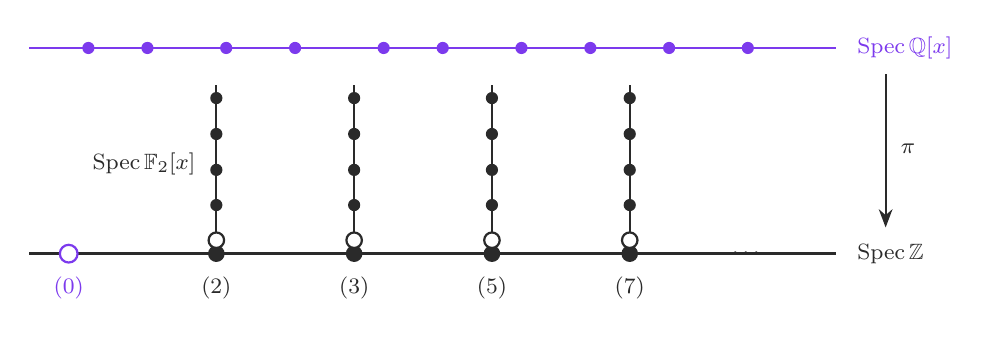
\begin{tikzpicture}[x=1.25cm, y=0.95cm, font=\footnotesize]
    %% --- Base: Spec Z ---
    \draw[very thick, chalkbody] (-0.1,0) -- (8.1,0);
    %% generic point (0): open circle in purple
    \draw[chalkpurple, thick, fill=white] (0.3,0) circle (3.2pt);
    \node[below=5pt, chalkpurple] at (0.3,0) {$(0)$};
    %% closed primes
    \foreach \x/\p in {1.8/{(2)}, 3.2/{(3)}, 4.6/{(5)}, 6.0/{(7)}} {
      \fill[chalkbody] (\x,0) circle (3pt);
      \node[below=5pt, chalkbody] at (\x,0) {$\p$};
    }
    \node[chalkbody] at (7.2,0) {$\cdots$};
    \node[right=4pt, chalkbody] at (8.1,0) {$\operatorname{Spec}\mathbb{Z}$};
    %% --- Special fibers (vertical lines over primes) ---
    \foreach \x in {1.8, 3.2, 4.6, 6.0} {
      \draw[thick, chalkbody] (\x,0.15) -- (\x,2.25);
      %% Type 3: open circle at base of fiber
      \draw[chalkbody, thick, fill=white] (\x,0.18) circle (2.8pt);
      %% Type 4: closed points on fiber
      \foreach \y in {0.65, 1.12, 1.60, 2.08} {
        \fill[chalkbody] (\x,\y) circle (2.2pt);
      }
    }
    %% label one fiber
    \node[left=4pt, chalkbody] at (1.8,1.2)
      {$\operatorname{Spec}\mathbb{F}_2[x]$};
    %% --- Generic fiber: Spec Q[x] ---
    \draw[thick, chalkpurple] (-0.1,2.75) -- (8.1,2.75);
    \foreach \x in {0.5,1.1,1.9,2.6,3.5,4.1,4.9,5.6,6.4,7.2} {
      \fill[chalkpurple] (\x,2.75) circle (2.2pt);
    }
    \node[right=4pt, chalkpurple] at (8.1,2.75)
      {$\operatorname{Spec}\mathbb{Q}[x]$};
    %% --- Projection arrow ---
    \draw[-{Stealth}, thick, chalkbody] (8.6,2.4) -- (8.6,0.35);
    \node[right=2pt, chalkbody] at (8.6,1.4) {$\pi$};
  \end{tikzpicture}
  \end{center}

  \vspace{-2pt}
  Each vertical slice is a copy of $\operatorname{Spec}\mathbb{F}_p[x]$;
  the top line is $\operatorname{Spec}\mathbb{Q}[x]$.
  These fibers are visible as \emph{sets} — but do they carry a natural
  \emph{scheme structure}?
\end{frame}

%% ----- Slide 6: Affine schemes -----------------------------------
\begin{frame}{Affine schemes — a minimal introduction}
  A \textbf{commutative ring} $A$ (e.g.\ $\mathbb{Z}$, $k[x]$, $\mathbb{Z}[x]$)
  determines a geometric object:
  \[
    \operatorname{Spec} A \;:=\; \{\text{prime ideals } \mathfrak{p} \subset A\}.
  \]

  \medskip

  \begin{itemize}
    \item A prime ideal $\mathfrak{p}$ is \emph{closed} if it is maximal;
          otherwise it is a \emph{generic point}, whose closure contains
          all primes that contain it.

    \smallskip

    \item \textbf{Example:} $\operatorname{Spec}\mathbb{Z}$ has one generic
          point $(0)$ and one closed point $(p)$ for each prime number $p$.

    \smallskip

    \item \textbf{Example:} $\operatorname{Spec}\mathbb{F}_p[x]$ has one generic
          point $(0)$ and one closed point $(q(x))$ for each monic irreducible
          $q \in \mathbb{F}_p[x]$ — this is the \emph{affine line over
          $\mathbb{F}_p$}.
  \end{itemize}
\end{frame}

%% ----- Slide 7: Ring maps and scheme maps ------------------------
\begin{frame}{Ring homomorphisms and morphisms of schemes}
  A ring homomorphism $\varphi : B \to A$ induces a map of schemes
  going \emph{the other way}:
  \[
    f = \operatorname{Spec}\varphi \;:\;
    \operatorname{Spec} A \;\longrightarrow\; \operatorname{Spec} B,
    \qquad
    \mathfrak{q} \;\longmapsto\; \varphi^{-1}(\mathfrak{q}).
  \]
  One checks that if $\mathfrak{q}$ is prime in $A$ then
  $\varphi^{-1}(\mathfrak{q})$ is prime in $B$.

  \bigskip

  \textbf{Our running example.}\enspace
  The inclusion $\iota : \mathbb{Z} \hookrightarrow \mathbb{Z}[x]$
  gives the projection
  \[
    \pi = \operatorname{Spec}\iota \;:\;
    \operatorname{Spec}\mathbb{Z}[x] \;\longrightarrow\; \operatorname{Spec}\mathbb{Z},
    \qquad
    \mathfrak{p} \;\longmapsto\; \mathfrak{p} \cap \mathbb{Z}.
  \]
  This is precisely the contraction $\mathfrak{p} \cap \mathbb{Z}$ from our
  case split — now seen as a morphism of schemes.
\end{frame}

%% ----- Slide 8: Localization -------------------------------------
\begin{frame}{Localization}
  Let $A$ be a ring and $S \subseteq A$ a \emph{multiplicative set}
  ($1 \in S$, closed under multiplication).
  The \textbf{localization} $S^{-1}A$ is the ring of formal fractions
  \[
    \frac{a}{s},\quad a \in A,\; s \in S,
  \]
  where $\dfrac{a}{s} = \dfrac{b}{t}$ iff $u(at - bs) = 0$ for some $u \in S$.

  \medskip

  \textbf{Key examples.}
  \begin{itemize}
    \item $A = \mathbb{Z}$,\; $S = \mathbb{Z}\setminus\{0\}$:\quad
          $S^{-1}\mathbb{Z} = \mathbb{Q}$.

    \item $A = \mathbb{Z}$,\; $S = \mathbb{Z}\setminus(p)$:\quad
          $S^{-1}\mathbb{Z} = \mathbb{Z}_{(p)}$
          (integers with denominators coprime to $p$).

    \item $A$ an \emph{integral domain},\;
          $S = A\setminus\{0\}$:\quad
          $S^{-1}A = \operatorname{Frac}(A)$, the fraction field.
  \end{itemize}

  \medskip
  The last example is what we need next:
  the \emph{residue field} at a prime will be the fraction field of a
  quotient domain.
\end{frame}

%% ----- Slide 9: The residue field --------------------------------
\begin{frame}{The residue field $\kappa(\mathfrak{p})$}
  Let $B$ be a ring and $\mathfrak{p} \in \operatorname{Spec} B$.
  The \textbf{residue field} at $\mathfrak{p}$ is
  \[
    \kappa(\mathfrak{p}) \;:=\; \operatorname{Frac}(B/\mathfrak{p}).
  \]
  It arises from a natural two-step factorization of $B \to \kappa(\mathfrak{p})$:
  \[
    B \;\xrightarrow{\;\text{quotient}\;}\; B/\mathfrak{p}
      \;\xrightarrow{\;\text{localize}\;}\;
      \operatorname{Frac}(B/\mathfrak{p}) \;=\; \kappa(\mathfrak{p}).
  \]

  \medskip

  \textbf{Examples for $B = \mathbb{Z}$.}
  \begin{itemize}
    \item $\mathfrak{p} = (0)$:\quad
          $\mathbb{Z}/(0) = \mathbb{Z}$,\;
          $\kappa((0)) = \operatorname{Frac}(\mathbb{Z}) = \mathbb{Q}$.

    \item $\mathfrak{p} = (p)$:\quad
          $\mathbb{Z}/(p) = \mathbb{F}_p$ is already a field,\;
          $\kappa((p)) = \mathbb{F}_p$.
  \end{itemize}

  \medskip
  These are exactly the fields whose spectra gave us the two fibers of
  $\pi : \operatorname{Spec}\mathbb{Z}[x] \to \operatorname{Spec}\mathbb{Z}$.
\end{frame}

%% ----- Slide 10: Spec κ(y) as the scheme-theoretic point --------
\begin{frame}{$\operatorname{Spec}\kappa(y)$ as the scheme-theoretic point}
  The ring map $B \to \kappa(\mathfrak{p})$ induces a morphism of schemes
  \[
    i_y \;:\; \operatorname{Spec}\kappa(y) \;\longrightarrow\; Y
      \;=\; \operatorname{Spec} B,
  \]
  whose image is the single point $\{y\}$.

  \medskip

  \textbf{Intuition.}\enspace
  $\operatorname{Spec}\kappa(y)$ is the \emph{scheme-theoretic incarnation}
  of the point $y$. To locate $y$ inside $Y$, the two steps do:
  \begin{itemize}
    \item \emph{Quotient} $B \to B/\mathfrak{p}$: cuts out the closed subscheme
          $\overline{\{y\}}$, the closure of $y$.
    \item \emph{Localize} $B/\mathfrak{p} \to \kappa(\mathfrak{p})$:
          pinpoints $y$ as the generic point of $\overline{\{y\}}$.
  \end{itemize}

  \medskip

  In other words: a point $y \in Y$ is the same data as a morphism
  $\operatorname{Spec}\kappa(y) \to Y$.
  This is the correct way to \emph{map a point into a scheme}.
\end{frame}

%% ----- Slide 11: Tensor products and fiber products -------------
\begin{frame}{The tensor product and the affine fiber product}
  Let $\varphi: B \to A$ and $\psi: B \to C$ be ring homomorphisms.
  The \textbf{tensor product} $A \otimes_B C$ is generated by symbols
  $a \otimes c$ subject to $B$-bilinearity:
  \[
    \varphi(b)\,a \otimes c \;=\; a \otimes \psi(b)\,c
    \qquad \text{for all } b \in B.
  \]

  \medskip

  \textbf{Key fact.}\enspace The fiber product of affine schemes over
  $\operatorname{Spec} B$ is:
  \begin{mathbox}
  \[
    \operatorname{Spec} A \times_{\operatorname{Spec} B} \operatorname{Spec} C
    \;=\; \operatorname{Spec}(A \otimes_B C).
  \]
  \end{mathbox}

  \medskip

  \textbf{Two examples we already know.}
  \begin{itemize}
    \item $\mathbb{Z}[x] \otimes_{\mathbb{Z}} \mathbb{Q}
          \;\cong\; \mathbb{Q}[x]$.
    \item $\mathbb{Z}[x] \otimes_{\mathbb{Z}} \mathbb{F}_p
          \;\cong\; \mathbb{F}_p[x]$.
  \end{itemize}
  These are the fibers of $\pi$ we computed at the start — now understood
  as tensor products.
\end{frame}

%% ----- Slide 12: Definition of the scheme-theoretic fiber -------
\begin{frame}{The scheme-theoretic fiber}
  Let $f : X \to Y$ be a morphism of schemes, $y \in Y$ a point.
  In the affine case $X = \operatorname{Spec} A$, $Y = \operatorname{Spec} B$,
  $f$ corresponds to $\varphi : B \to A$.

  \medskip

  \textbf{Definition.}\enspace The \textbf{scheme-theoretic fiber} of $f$
  over $y$ is the fiber product
  \begin{mathbox}
  \[
    X_y \;:=\; X \times_Y \operatorname{Spec}\kappa(y)
         \;=\; \operatorname{Spec}\!\bigl(A \otimes_B \kappa(\mathfrak{p})\bigr).
  \]
  \end{mathbox}

  \medskip

  \textbf{What we still need to check.}\enspace
  The set of prime ideals of $A \otimes_B \kappa(\mathfrak{p})$ should be
  exactly the set-theoretic fiber:
  \[
    \bigl\{\,\mathfrak{q} \in \operatorname{Spec} A
    \;\bigm|\; \varphi^{-1}(\mathfrak{q}) = \mathfrak{p}\,\bigr\}.
  \]
  This is what we verify on the next slides using the two-step factorization
  $B \to B/\mathfrak{p} \to \kappa(\mathfrak{p})$.
\end{frame}

%% ----- Slide 13: The quotient step ------------------------------
\begin{frame}{Step 1 of 2: the quotient}
  The factorization $B \to B/\mathfrak{p} \to \kappa(\mathfrak{p})$
  splits the computation of $A \otimes_B \kappa(\mathfrak{p})$ into two steps.

  \medskip

  \textbf{First step} — tensor with $B/\mathfrak{p}$:
  \[
    A \otimes_B B/\mathfrak{p} \;\cong\; A/\mathfrak{p}^e,
  \]
  where $\mathfrak{p}^e := \varphi(\mathfrak{p})\cdot A$ is the
  \emph{extended ideal} of $\mathfrak{p}$ in $A$.
  (This follows from right-exactness of $\otimes$
  applied to $\mathfrak{p} \to B \to B/\mathfrak{p} \to 0$.)

  \medskip

  \textbf{Geometric meaning.}\enspace
  $\operatorname{Spec}(A/\mathfrak{p}^e) = f^{-1}\!\bigl(\overline{\{y\}}\bigr)$,
  the scheme-theoretic preimage of the \emph{closure} of $y$.

  \medskip

  \textbf{Which primes survive?}\enspace
  The primes of $A/\mathfrak{p}^e$ are those
  $\mathfrak{q} \in \operatorname{Spec} A$ satisfying
  \[
    \varphi^{-1}(\mathfrak{q}) \;\supseteq\; \mathfrak{p}.
  \]
  This is too broad — it includes primes over proper specializations of
  $\mathfrak{p}$. The localization step will cut those out.
\end{frame}

%% ----- Slide 14: The localization step --------------------------
\begin{frame}{Step 2 of 2: the localization}
  \textbf{Second step} — localize $A/\mathfrak{p}^e$ at
  $S = \varphi(B \setminus \mathfrak{p})$:
  \[
    S^{-1}(A/\mathfrak{p}^e)
    \;\cong\;
    (A/\mathfrak{p}^e) \otimes_{B/\mathfrak{p}} \kappa(\mathfrak{p})
    \;\cong\;
    A \otimes_B \kappa(\mathfrak{p}).
  \]

  \medskip

  \textbf{Effect.}\enspace Localization at $S$ kills every prime
  $\mathfrak{q} \subset A/\mathfrak{p}^e$ that meets $S$,
  i.e.\ every $\mathfrak{q}$ for which
  $\mathfrak{q} \cap \varphi(B\setminus\mathfrak{p}) \neq \emptyset$,
  equivalently
  \[
    \varphi^{-1}(\mathfrak{q}) \;\not\subseteq\; \mathfrak{p}.
  \]
  Only the primes with $\varphi^{-1}(\mathfrak{q}) \subseteq \mathfrak{p}$
  survive.

  \medskip

  \textbf{Geometric meaning.}\enspace
  We are shrinking from the preimage of $\overline{\{y\}}$ down to the
  preimage of the generic point of $\overline{\{y\}}$ — which is $y$ itself.
\end{frame}

%% ----- Slide 15: Both conditions together — the table -----------
\begin{frame}{The two conditions together}
  A prime $\mathfrak{q} \in \operatorname{Spec} A$ survives both operations
  iff it satisfies both constraints simultaneously:
  \[
    \varphi^{-1}(\mathfrak{q}) \supseteq \mathfrak{p}
    \quad\text{and}\quad
    \varphi^{-1}(\mathfrak{q}) \subseteq \mathfrak{p}
    \quad\Longrightarrow\quad
    \varphi^{-1}(\mathfrak{q}) = \mathfrak{p}.
  \]

  \medskip

  \renewcommand{\arraystretch}{1.5}
  \begin{tabular}{@{\hspace{4pt}}lll@{\hspace{4pt}}}
    \toprule
    \textbf{Operation} & \textbf{Algebra} & \textbf{Primes kept} \\
    \midrule
    Quotient  & $A \to A/\mathfrak{p}^e$
              & $\varphi^{-1}(\mathfrak{q}) \supseteq \mathfrak{p}$ \\
    Localize  & $A/\mathfrak{p}^e \to S^{-1}(A/\mathfrak{p}^e)$
              & $\varphi^{-1}(\mathfrak{q}) \subseteq \mathfrak{p}$ \\
    \midrule
    \textbf{Combined} & $A \to A \otimes_B \kappa(\mathfrak{p})$
              & $\varphi^{-1}(\mathfrak{q}) = \mathfrak{p}$ \\
    \bottomrule
  \end{tabular}

  \medskip

  The underlying set of $\operatorname{Spec}(A \otimes_B \kappa(\mathfrak{p}))$
  is the set-theoretic fiber $f^{-1}(y)$, now equipped with a natural
  scheme structure.
\end{frame}

%% ----- Slide 16: Back to Spec Z[x] — the fibers ----------------
\begin{frame}{Back to $\operatorname{Spec}\mathbb{Z}[x]$: computing the fibers}
  Apply the machinery to $\varphi : \mathbb{Z} \hookrightarrow \mathbb{Z}[x]$.

  \bigskip

  \textbf{Generic fiber} over $(0) \in \operatorname{Spec}\mathbb{Z}$:
  \[
    \kappa((0)) = \mathbb{Q},
    \qquad
    \mathbb{Z}[x] \otimes_{\mathbb{Z}} \mathbb{Q} \;\cong\; \mathbb{Q}[x].
  \]
  The fiber is $\operatorname{Spec}\mathbb{Q}[x]$, the affine line over $\mathbb{Q}$.

  \bigskip

  \textbf{Special fiber} over $(p) \in \operatorname{Spec}\mathbb{Z}$:
  \[
    \kappa((p)) = \mathbb{F}_p,
    \qquad
    \mathbb{Z}[x] \otimes_{\mathbb{Z}} \mathbb{F}_p \;\cong\; \mathbb{F}_p[x].
  \]
  The fiber is $\operatorname{Spec}\mathbb{F}_p[x]$, the affine line over $\mathbb{F}_p$.

  \bigskip

  The case split from Slide 3 was always this: each case corresponds to
  a fiber, and the \emph{passage to $\mathbb{Q}[x]$ or $\mathbb{F}_p[x]$} is
  exactly the base change $\mathbb{Z}[x] \otimes_{\mathbb{Z}} \kappa(\mathfrak{p})$.
\end{frame}

%% ----- Slide 17: Four types revisited ---------------------------
\begin{frame}{The four types, revisited}
  Each prime of $\operatorname{Spec}\mathbb{Z}[x]$ lives in exactly one fiber,
  and plays a definite role within it.

  \medskip

  \renewcommand{\arraystretch}{1.55}
  \begin{tabular}{@{\hspace{4pt}}clll@{\hspace{4pt}}}
    \toprule
    \textbf{Type} & \textbf{Prime}
      & \textbf{Fiber $\mathbb{Z}[x]\otimes_{\mathbb{Z}}\kappa(\cdot)$}
      & \textbf{Role in fiber} \\
    \midrule
    1 & $(0)$
      & $\operatorname{Spec}\mathbb{Q}[x]$
      & Generic point \\
    2 & $(q(x))$, $q$ irred.\ prim.
      & $\operatorname{Spec}\mathbb{Q}[x]$
      & Closed point $(q)$ \\
    3 & $(p)$, $p$ prime
      & $\operatorname{Spec}\mathbb{F}_p[x]$
      & Generic point \\
    4 & $(p,q(x))$, $q$ irred.\ mod $p$
      & $\operatorname{Spec}\mathbb{F}_p[x]$
      & Closed point $(\bar{q})$ \\
    \bottomrule
  \end{tabular}

  \medskip

  Types 1 and 2 belong to the \emph{generic fiber};
  Types 3 and 4 to a \emph{special fiber over $p$}.
  The case split from the beginning was always a fiber-by-fiber analysis.
\end{frame}

%% ----- Slide 18: Specialization ---------------------------------
\begin{frame}{Specialization: how fibers meet}
  A prime $\mathfrak{q}'$ is a \textbf{specialization} of $\mathfrak{q}$ if
  $\mathfrak{q} \subsetneq \mathfrak{q}'$, i.e.\ $\mathfrak{q}'$ lies
  in the closure of $\mathfrak{q}$ in the Zariski topology.

  \medskip

  \textbf{In $\operatorname{Spec}\mathbb{Z}[x]$.}
  A Type 2 prime $(q(x))$ specializes to a Type 4 prime $(p,\,\bar{q}(x))$
  precisely when $\bar{q}(x) = q(x) \bmod p$ is still irreducible over
  $\mathbb{F}_p$.
  \begin{itemize}
    \item If $q(x)$ factors mod $p$, its specialization splits across
          \emph{several} Type 4 primes — this is the geometric shadow of
          prime factorization in $\mathbb{F}_p[x]$.
    \item If $q(x)$ has a repeated factor mod $p$, the fiber over $p$ is
          \emph{ramified} — a phenomenon central to algebraic number theory.
  \end{itemize}

  \medskip

  The fiber product computes \emph{which} primes land in each fiber;
  specialization tells us how fibers relate to one another across $\operatorname{Spec}\mathbb{Z}$.
\end{frame}

%% ----- Slide 19: Base change / reduction mod p ------------------
\begin{frame}{Base change: reduction mod $p$}
  The fiber product $X \times_Y \operatorname{Spec}\kappa(y)$
  is also called the \textbf{base change} of $X$ along $i_y$.
  It turns a scheme over $Y$ into a scheme over the single point $\kappa(y)$.

  \medskip

  \textbf{For $\operatorname{Spec}\mathbb{Z}[x]$.}\enspace
  Given a polynomial $f \in \mathbb{Z}[x]$, the zero locus
  $V(f) \subset \operatorname{Spec}\mathbb{Z}[x]$ is a scheme over
  $\operatorname{Spec}\mathbb{Z}$.
  Its fibers are:
  \begin{itemize}
    \item $V(f) \times_{\operatorname{Spec}\mathbb{Z}} \operatorname{Spec}\mathbb{Q}
          \;=\; \operatorname{Spec}\mathbb{Q}[x]/(f)$
          \quad — roots of $f$ over $\mathbb{Q}$.
    \item $V(f) \times_{\operatorname{Spec}\mathbb{Z}} \operatorname{Spec}\mathbb{F}_p
          \;=\; \operatorname{Spec}\mathbb{F}_p[x]/(\bar{f})$
          \quad — roots of $f \bmod p$.
  \end{itemize}

  \medskip

  \textbf{Slogan.}\enspace \emph{Reduction mod $p$ is base change to the
  special fiber.}
  The fiber product is the precise algebraic meaning of this operation.
\end{frame}

\iffalse  %% ---- commented-out future directions (slides 20–23) ----
%% ----- Slide 20: General fiber products -------------------------
\begin{frame}{Future direction I: beyond affine schemes}
  Everything so far was for $\operatorname{Spec} A$.
  General schemes are built by \emph{gluing} affine pieces along open subsets.

  \medskip

  \textbf{The gluing construction.}\enspace
  Given schemes $X$, $Y$, $S$ with morphisms $X \to S \leftarrow Y$,
  the fiber product $X \times_S Y$ is constructed by covering $X$, $Y$, $S$
  with affine opens, taking affine fiber products on each overlap, and
  gluing the results.

  \medskip

  \textbf{Key properties that survive.}
  \begin{itemize}
    \item The universal property still holds: morphisms $T \to X \times_S Y$
          correspond bijectively to pairs of morphisms $T \to X$, $T \to Y$
          over $S$.
    \item The scheme-theoretic fiber $f^{-1}(y) = X \times_Y \operatorname{Spec}\kappa(y)$
          is defined identically — it does not require affineness.
    \item Affine fiber products remain the local model: every fiber product
          computation reduces to tensor products on affine patches.
  \end{itemize}
\end{frame}

%% ----- Slide 21: Ramification -----------------------------------
\begin{frame}{Future direction II: ramification}
  The fiber product sees more than just which points lie over $p$ —
  it detects the \emph{scheme structure} of the fiber, including
  phenomena invisible at the level of sets.

  \medskip

  \textbf{Example.}\enspace
  Let $f = x^2 - p \in \mathbb{Z}[x]$.
  The special fiber over $(p)$ is
  \[
    \operatorname{Spec}\mathbb{F}_p[x]/(x^2)
    \;\cong\;
    \operatorname{Spec}\mathbb{F}_p[x]/(x)^2.
  \]
  As a \emph{set} this is a single point.
  But as a \emph{scheme} it is non-reduced: the ring $\mathbb{F}_p[x]/(x^2)$
  has a nilpotent element $x$.

  \medskip

  This non-reducedness is \textbf{ramification}.
  It is the algebraic-geometric incarnation of the fact that $p$ ramifies
  in $\mathbb{Z}[\sqrt{p}]$ — and it is precisely what the fiber product,
  rather than the set-theoretic fiber, captures.
\end{frame}

%% ----- Slide 22: Cohomology and base change ---------------------
\begin{frame}{Future direction III: cohomology and base change}
  Once fiber products are in hand, one can ask:
  if $f : X \to Y$ is a morphism and $y : \operatorname{Spec}\kappa(y) \to Y$
  a point, how does the cohomology of $\mathcal{F}$ on $X$ relate to the
  cohomology of its restriction $\mathcal{F}|_{X_y}$ on the fiber?

  \medskip

  \textbf{Base change maps.}\enspace There are natural maps
  \[
    H^i(X,\,\mathcal{F}) \otimes_{\mathcal{O}_{Y,y}} \kappa(y)
    \;\longrightarrow\;
    H^i(X_y,\,\mathcal{F}|_{X_y}),
  \]
  which ask whether cohomology commutes with passing to fibers.

  \medskip

  \textbf{The theorems.}
  \begin{itemize}
    \item \emph{Flat base change}: the maps are isomorphisms when
          $f$ is flat and $\mathcal{F}$ is flat over $Y$.
    \item \emph{Proper base change}: for proper $f$ and constructible
          $\mathcal{F}$, cohomology commutes with arbitrary base change
          on the \'etale site.
  \end{itemize}
  These are central tools in modern algebraic geometry and number theory.
\end{frame}

%% ----- Slide 23: Arithmetic surfaces ----------------------------
\begin{frame}{Future direction IV: arithmetic surfaces}
  $\operatorname{Spec}\mathbb{Z}[x]$ is the prototype of an
  \textbf{arithmetic surface}: a two-dimensional scheme fibered over
  $\operatorname{Spec}\mathbb{Z}$, with a curve in every fiber.

  \medskip

  \textbf{The general picture.}\enspace
  Replace $\mathbb{Z}[x]$ by the coordinate ring of a curve $C$ over $\mathbb{Z}$
  (e.g.\ an elliptic curve $y^2 = x^3 + ax + b$).
  The fibers are:
  \begin{itemize}
    \item \emph{Generic fiber}: $C$ as a curve over $\mathbb{Q}$ —
          the object of classical Diophantine geometry.
    \item \emph{Special fiber over $p$}: the reduction $C \bmod p$,
          which may be smooth, nodal, or cuspidal.
  \end{itemize}

  \medskip

  The interplay between the generic and special fibers —
  how singularities in the special fiber reflect arithmetic of the
  generic fiber — is the central theme of
  \emph{N\'eron models}, \emph{Arakelov geometry}, and ultimately the
  geometric side of the proof of Fermat's Last Theorem.
\end{frame}

\fi  %% ---- end commented-out section ----------------------------

%% ----- Slide 20: Two philosophies of geometry -------------------
\begin{frame}{Two philosophies: charts versus algebra}
  \textbf{Complex geometry.}\enspace
  A complex manifold is built chart by chart.
  \begin{itemize}
    \item Cover $X$ by open sets $U_\alpha \cong \mathbb{C}^n$.
    \item Write down transition functions $\varphi_{\alpha\beta}$ on overlaps.
    \item Define a bundle by local trivializations satisfying the cocycle
          condition on triple overlaps.
    \item Define a section by compatible local data on each chart.
  \end{itemize}
  \emph{The local picture is primary.
  The global picture is assembled from it.}

  \bigskip

  \textbf{Algebraic geometry.}\enspace
  Start with a single global algebraic object — a ring, a graded ring,
  a sheaf.
  \begin{itemize}
    \item The local picture is \emph{derived}: apply localization at a
          prime to zoom in near a point.
    \item No coordinates to choose, no transition functions to verify.
  \end{itemize}
  \emph{The global picture is primary.
  Localization hands you the local data for free.}
\end{frame}

%% ----- Slide 21: The structure sheaf ----------------------------
\begin{frame}{The structure sheaf: sections without coordinates}
  On a complex manifold $X$, the \textbf{structure sheaf} $\mathcal{O}_X$
  assigns to each open $U \subset X$ the ring of holomorphic functions
  $\mathcal{O}_X(U)$, with restriction maps for $V \subset U$.

  \medskip

  The same definition works on any scheme.
  On $\operatorname{Spec} A$:
  \[
    \mathcal{O}_X(D(f)) \;=\; A_f
    \qquad \text{(localization of $A$ at $f$).}
  \]
  No coordinates — the ring $A$ is the global data;
  the local rings $A_f$ are derived from it by localization.

  \medskip

  A \textbf{sheaf} $\mathcal{F}$ on $X$ is a rule assigning a module
  $\mathcal{F}(U)$ to each open $U$, compatible with restrictions,
  satisfying a gluing condition.
  It is the algebraic replacement for a holomorphic vector bundle
  — but defined globally, not chart by chart.

  \medskip

  \textbf{The key shift.}\enspace
  In complex geometry a bundle is a collection of local pieces that agree.
  In algebraic geometry a sheaf is a single global object that localizes.
\end{frame}

%% ----- Slide 22: Graded rings — the algebra of weights ----------
\begin{frame}{Graded rings: algebra remembers scaling}
  A \textbf{graded ring} is a ring with a decomposition
  \[
    S \;=\; S_0 \oplus S_1 \oplus S_2 \oplus \cdots,
    \qquad S_i \cdot S_j \;\subset\; S_{i+j}.
  \]
  An element of $S_d$ is said to have \emph{degree $d$}.

  \medskip

  \textbf{For a complex geometer.}\enspace
  The grading encodes a $\mathbb{C}^*$-action:
  an element $f \in S_d$ transforms as
  $f \mapsto \lambda^d f$ under $\lambda \in \mathbb{C}^*$.
  This is exactly the action of $\mathbb{C}^*$ on
  $\mathbb{C}^{n+1} \setminus \{0\}$ by scalar multiplication —
  the action whose quotient is $\mathbb{P}^n$.

  \medskip

  \textbf{Prototype.}\enspace
  $S = k[x_0, \ldots, x_n]$ with $\deg x_i = 1$.
  The degree-$d$ piece $S_d$ is spanned by monomials of total degree $d$.
  The ring encodes how homogeneous polynomials transform under scaling.

  \medskip

  \textbf{The point.}\enspace
  Wherever a $\mathbb{C}^*$-action appears geometrically,
  a graded ring appears algebraically.
  $\operatorname{Proj}(S)$ is the algebraic way to take the quotient
  by that action.
\end{frame}

%% ----- Slide 23: Graded algebras beyond polynomials -------------
\begin{frame}{Two graded algebras from a closed embedding}
  Let $Y = \operatorname{Spec} A$ and $X = V(I) \subset Y$ a closed
  subscheme.
  Two graded algebras arise naturally:

  \medskip

  \textbf{Associated graded} $\operatorname{gr}_I(A)
    = \bigoplus_{n \geq 0} I^n/I^{n+1}$.

  Elements are \emph{leading terms} along $X$:
  a function $a \in I^n \setminus I^{n+1}$ vanishes to exact order $n$,
  and its image in $I^n/I^{n+1}$ is its tangential part.
  Geometrically: $\operatorname{Spec}(\operatorname{gr}_I(A))$
  is the \textbf{normal cone} $C_X Y$.

  \smallskip

  \textbf{Rees algebra} $\operatorname{Rees}(I)
    = \bigoplus_{n \geq 0} I^n t^n \subset A[t]$.

  Encodes the full filtration, not just the leading terms.
  Geometrically: $\operatorname{Proj}(\operatorname{Rees}(I))$
  is the \textbf{blow-up} $\operatorname{Bl}_X Y$ — the scheme that
  separates directions of approach to $X$.

  \medskip

  \textbf{Punchline.}\enspace
  A single closed embedding $X \hookrightarrow Y$ produces two canonical
  graded algebras.
  Applying $\operatorname{Proj}$ turns them into geometric objects —
  no coordinates chosen at any step.
\end{frame}

%% ----- Slide 24: Proj(S) ----------------------------------------
\begin{frame}{$\operatorname{Proj}(S)$: projective space without coordinates}
  Let $S = \bigoplus_{n \geq 0} S_n$ be a graded ring.
  Define
  \[
    \operatorname{Proj}(S) \;:=\;
    \{\,\text{homogeneous prime ideals } \mathfrak{p} \subset S
    \;\mid\; \mathfrak{p} \not\supset S_+\,\},
  \]
  where $S_+ = \bigoplus_{n \geq 1} S_n$ is the \emph{irrelevant ideal}.

  \medskip

  \textbf{The affine cover.}\enspace
  For any homogeneous $f \in S_+$, the locus $D_+(f) = \{\mathfrak{p} : f \notin \mathfrak{p}\}$
  is an affine open:
  \[
    D_+(f) \;\cong\; \operatorname{Spec}(S_{(f)}),
    \qquad
    S_{(f)} = \Bigl\{\,\tfrac{g}{f^n} : g \in S_n\Bigr\}.
  \]

  \textbf{Example: $\mathbb{P}^1_k = \operatorname{Proj}(k[s,t])$.}
  \begin{itemize}
    \item $D_+(s) \cong \operatorname{Spec}(k[t/s]) = \mathbb{A}^1_k$.
    \item $D_+(t) \cong \operatorname{Spec}(k[s/t]) = \mathbb{A}^1_k$.
    \item Overlap: $D_+(st) \cong \operatorname{Spec}(k[t/s,(t/s)^{-1}]) = \mathbb{A}^1 \setminus \{0\}$.
  \end{itemize}
  The transition function $t/s \mapsto s/t$ is automatic from the algebra.
  \emph{No coordinate patch was chosen.}
\end{frame}

%% ----- Slide 25: Why ℙ¹ is not affine --------------------------
\begin{frame}{Why $\mathbb{P}^1$ is not affine — and why that is fine}
  Suppose $\mathbb{P}^1_k = \operatorname{Spec} A$ for some ring $A$.
  Then $A = \mathcal{O}(\mathbb{P}^1) = H^0(\mathbb{P}^1, \mathcal{O})$.

  \medskip

  But a global regular function on $\mathbb{P}^1$ is a rational function
  with no poles anywhere — hence a constant.
  So $A = k$, and $\operatorname{Spec} k$ is a single point.
  Contradiction.

  \medskip

  \textbf{What $\operatorname{Proj}$ does instead.}\enspace
  The graded ring $k[s,t]$ is global data for $\mathbb{P}^1$,
  but it is \emph{not} the ring of global functions — it is the ring of
  sections of all line bundles $\mathcal{O}(d)$ at once:
  \[
    k[s,t]_d \;=\; H^0(\mathbb{P}^1, \mathcal{O}(d)).
  \]
  The non-affineness of $\mathbb{P}^1$ reflects its \emph{compactness}
  (no non-constant bounded functions).
  $\operatorname{Proj}$ is the correct algebraic notion of compactness —
  the analog of a compact complex manifold.
\end{frame}

%% ----- Slide 26: Direct image sheaf — definition ----------------
\begin{frame}{The direct image sheaf: one definition, no coordinates}
  Let $f : X \to Y$ be a morphism of schemes and $\mathcal{F}$ a sheaf
  on $X$.
  The \textbf{direct image} $f_*\mathcal{F}$ is the sheaf on $Y$ defined by
  \begin{mathbox}
    \[
      (f_*\mathcal{F})(U) \;:=\; \mathcal{F}(f^{-1}(U))
      \qquad \text{for every open } U \subset Y.
    \]
  \end{mathbox}
  Restriction maps: $f^{-1}(V) \subset f^{-1}(U)$ for $V \subset U$,
  so restriction of $\mathcal{F}$ gives the required map.
  The sheaf axioms for $f_*\mathcal{F}$ follow immediately from those
  of $\mathcal{F}$ — since $f^{-1}$ commutes with unions and intersections.

  \medskip

  \textbf{Compare with complex geometry.}\enspace
  To define the "bundle of fiber cohomologies" $R^0 f_* \mathcal{L}$
  on a holomorphic family, one needs harmonic theory, $L^2$ metrics,
  and Hodge theory to identify global sections fiber by fiber.
  Here: one line, no analysis, no metrics.
  The algebra does the same job globally.
\end{frame}

%% ----- Slide 27: Affine case and connection to fiber products ---
\begin{frame}{The affine case: restriction of scalars}
  Let $f : \operatorname{Spec} A \to \operatorname{Spec} B$ correspond to
  $\varphi : B \to A$, and let $\mathcal{F} = \widetilde{M}$ for an
  $A$-module $M$.

  \medskip

  \textbf{Claim.}\enspace
  $f_*\widetilde{M} \;\cong\; \widetilde{M_B}$,
  where $M_B$ is $M$ viewed as a $B$-module via $\varphi$.
  \emph{The pushforward is restriction of scalars} — forget the
  $A$-structure, keep only the $B$-structure.

  \medskip

  \textbf{The fiber, revisited.}\enspace
  The fiber of $f_*\widetilde{M}$ at $\mathfrak{p} \in \operatorname{Spec} B$ is
  \[
    (f_*\widetilde{M})\big|_{\mathfrak{p}}
    \;=\; M_B \otimes_B \kappa(\mathfrak{p})
    \;=\; M \otimes_A \mathcal{O}_{X_{\mathfrak{p}}},
  \]
  where $X_{\mathfrak{p}} = \operatorname{Spec}(A \otimes_B \kappa(\mathfrak{p}))$
  is the scheme-theoretic fiber we constructed earlier.

  \medskip

  The direct image closes the loop:
  the fiber of $f_*\mathcal{F}$ over a point $y$ is precisely
  $\mathcal{F}$ restricted to the fiber product
  $X \times_Y \operatorname{Spec}\kappa(y)$.
\end{frame}

%% ----- Slide 28: Example — ℙ¹-bundle over 𝔸¹ ------------------
\begin{frame}{Example: $\mathbb{P}^1$-bundle over $\mathbb{A}^1$}
  Let $B = k[t]$, $X = \mathbb{P}^1_B = \operatorname{Proj}(B[s_0, s_1])$,
  and $f : X \to \operatorname{Spec} B = \mathbb{A}^1$.
  Every fiber $f^{-1}(t_0) = \mathbb{P}^1_k$.

  \medskip

  \textbf{The direct image of $\mathcal{O}(d)$.}\enspace
  The degree-$d$ piece of the graded ring is
  \[
    H^0\!\bigl(\mathbb{P}^1_B,\,\mathcal{O}(d)\bigr)
    \;=\; \bigoplus_{j=0}^{d} B\cdot s_0^j s_1^{d-j}
    \;\cong\; B^{d+1}.
  \]
  Therefore $f_*\mathcal{O}(d) \cong \mathcal{O}_{\mathbb{A}^1}^{d+1}$:
  a free rank-$(d+1)$ sheaf on the base.

  \medskip

  \textbf{Checking the fiber.}\enspace At any point $t_0 \in \mathbb{A}^1$:
  \[
    \bigl(f_*\mathcal{O}(d)\bigr)\big|_{t_0}
    \;=\; B^{d+1} \otimes_{k[t]} k
    \;=\; k^{d+1}
    \;=\; H^0\!\bigl(\mathbb{P}^1_k,\,\mathcal{O}(d)\bigr).
  \]
  The direct image packages the cohomology of \emph{every} fiber into a
  single algebraic object on the base.
  Tensoring with $\kappa(t_0)$ recovers any individual fiber — no
  integration, no $L^2$ theory required.
\end{frame}

%% ----- Slide 29: The line bundle O(1) on Proj -------------------
\begin{frame}{The tautological line bundle $\mathcal{O}(1)$ on $\operatorname{Proj}(S)$}
  On $\mathbb{P}^n = \operatorname{Proj}(k[x_0,\ldots,x_n])$, the sheaf
  $\mathcal{O}(d)$ is defined by its sections on basic opens:
  \[
    \mathcal{O}(d)\bigl(D_+(f)\bigr)
    \;:=\; \Bigl\{\,\tfrac{g}{f^m} : g \in S_{d + m\deg f}\Bigr\}.
  \]
  Geometrically: $\mathcal{O}(1)$ is the \emph{hyperplane line bundle} —
  its global sections are exactly the linear forms $\sum a_i x_i$.

  \medskip

  \textbf{Key properties.}
  \begin{itemize}
    \item $H^0(\mathbb{P}^n, \mathcal{O}(d)) = S_d$ for $d \geq 0$:
          global sections are degree-$d$ homogeneous polynomials.
    \item $\mathcal{O}(1)$ is \emph{ample}: its powers
          $\mathcal{O}(d)$ embed $\mathbb{P}^n$ into projective space.
    \item For any $\operatorname{Proj}(S)$, the same construction gives a
          tautological $\mathcal{O}(1)$ encoding the grading.
  \end{itemize}

  \medskip

  The same idea applies to $\operatorname{Proj}(\operatorname{Rees}(I))$
  and $\operatorname{Proj}(\operatorname{gr}_I(A))$ — the blow-up and the
  normal cone both carry natural line bundles inherited from the grading.
\end{frame}

%% ================================================================
%%  PART II — DEFORMATION TO THE NORMAL CONE
%% ================================================================

%% ----- Slide 30: The extended Rees algebra ----------------------
\begin{frame}{The extended Rees algebra}
  The standard Rees algebra $\bigoplus_{n \geq 0} I^n t^n$ lives over $\mathbb{A}^1_t$,
  but has no well-behaved fiber at $t = \infty$.
  The fix: extend the grading to all integers.

  \medskip

  \textbf{Definition.}\enspace Set $u = t^{-1}$ (the deformation parameter).
  The \textbf{extended Rees algebra} is
  \[
    R'(I) \;=\; \bigoplus_{n \in \mathbb{Z}} I^n u^{-n} \;\subset\; A[u, u^{-1}],
    \qquad I^n := A \;\text{ for } n \leq 0.
  \]

  \medskip

  \textbf{Two structural facts.}
  \begin{itemize}
    \item \textbf{At $u = 0$:}\enspace
          $R'(I)/(u) \;\cong\; \operatorname{gr}_I(A) = \bigoplus_{n \geq 0} I^n/I^{n+1}$.
    \item \textbf{Away from $u = 0$:}\enspace
          $R'(I)[u^{-1}] = A[u, u^{-1}]$ — the filtration by $I$ vanishes
          once $u$ is invertible.
  \end{itemize}

  \medskip

  \textbf{Note.}\enspace Since $I \subsetneq A$ is proper, $u^{-1} = t \notin R'(I)$:
  the degree-$1$ piece is $I \cdot u^{-1}$, not $A \cdot u^{-1}$.
  So $R'(I)$ is an $A[u]$-algebra — the family lives over $\mathbb{A}^1_u$, not $\mathbb{G}_m$.
\end{frame}

%% ----- Slide 31: The flat family --------------------------------
\begin{frame}{The flat family over $\mathbb{A}^1$}
  The inclusion $A[u] \hookrightarrow R'(I)$ makes
  \[
    \mathcal{M} \;=\; \operatorname{Spec}(R'(I))
    \;\longrightarrow\;
    Y \times \mathbb{A}^1_u \;=\; \operatorname{Spec}(A[u])
  \]
  a \textbf{flat} morphism — the deformation of $Y$ to the normal cone of $X$.

  \medskip

  \renewcommand{\arraystretch}{1.45}
  \begin{tabular}{@{\hspace{4pt}}lll@{\hspace{4pt}}}
    \toprule
    \textbf{Locus} & \textbf{Fiber} & \textbf{Ring} \\
    \midrule
    $u \neq 0$ & $Y = \operatorname{Spec}(A)$ \enspace (constant)
               & $R'(I)[u^{-1}] = A[u, u^{-1}]$ \\
    $u = 0$    & $C_X Y$ \enspace (normal cone)
               & $R'(I)/(u) \cong \operatorname{gr}_I(A)$ \\
    \bottomrule
  \end{tabular}

  \smallskip

  \textbf{Why flatness matters.}\enspace
  A flat family preserves the cycle class of its fibers.
  Consequently $[Y]$ and $[C_X Y]$ are \emph{rationally equivalent} cycles —
  they are fibers of a flat family over $\mathbb{A}^1$
  (compactified to $\mathbb{P}^1$ in slide 33),
  hence differ by a boundary in the Chow group.
  This is precisely what makes the specialization map
  $\sigma : A_k(Y) \to A_k(C_X Y)$ well-defined.
\end{frame}

%% ----- Slide 32: Why the special fiber sees only leading terms --
\begin{frame}{The special fiber sees only leading terms}
  Let $a \in I^n \setminus I^{n+1}$: we say $a$ has \textbf{order $n$ along $X$}.

  \medskip

  \begin{itemize}
    \item \textbf{In $R'(I)$:}\enspace
          $a$ appears at $u$-degree $-k$ for $k = 0, 1, \ldots, n$
          (as $a \cdot u^{-k} \in I^k \cdot u^{-k}$),
          but \emph{not} at degree $-(n+1)$, since $a \notin I^{n+1}$.
          So $-n$ is the most negative degree at which $a$ appears.

    \smallskip

    \item \textbf{Setting $u = 0$:}\enspace
          the degree-$(-k)$ piece of $R'(I)/(u)$ is $I^k/I^{k+1}$.
          For $k < n$: $a \in I^k$ but the quotient kills it (it is not
          in $I^k \setminus I^{k+1}$). At $k = n$: $a$ maps to
          $[a] \in I^n/I^{n+1}$ — its \emph{leading term} — which is nonzero.
  \end{itemize}

  \medskip

  \begin{mathbox}
    $C_X Y = \operatorname{Spec}(\operatorname{gr}_I(A))$ is the
    \textbf{scheme of leading terms}: for each $a \in A$,
    only the lowest-order part of $a$ along $I$ survives in the special fiber.
    It is the algebraic tangent cone to $Y$ along $X$.
  \end{mathbox}
\end{frame}

%% ----- Slide 33: Normal cone, blow-up, and the big picture ------
\begin{frame}{Normal cone, blow-up, and the deformation picture}
  Two canonical schemes arise from the closed embedding $X \hookrightarrow Y$:

  \medskip

  \begin{itemize}
    \item \textbf{Normal cone:}\enspace
          $C_X Y = \operatorname{Spec}(\operatorname{gr}_I(A))$.
          The grading gives a $\mathbb{G}_m$-action on $C_X Y$ over $X$
          — this is what makes it a \emph{cone}.

    \smallskip

    \item \textbf{Blow-up:}\enspace
          $\operatorname{Bl}_X Y = \operatorname{Proj}(\operatorname{Rees}(I))$,
          with exceptional divisor
          \[
            E = \operatorname{Proj}(\operatorname{gr}_I(A)) = \mathbb{P}(C_X Y).
          \]
          Outside $E$, the blow-up is isomorphic to $Y \setminus X$.
  \end{itemize}

  \medskip

  \textbf{The interpolation.}\enspace
  Let $M^\circ = \mathcal{M} \setminus \widetilde{Y}$
  (remove the blow-up component from the special fiber).
  Then $M^\circ \to \mathbb{P}^1$ is a flat family:
  \[
    \text{fiber over } u \neq 0 :\; X \hookrightarrow Y,
    \qquad
    \text{fiber over } u = 0 :\; X \hookrightarrow C_X Y
    \;(\text{zero section}).
  \]
  \emph{The normal cone is the limit of $Y$ as we zoom toward $X$
  — the first-order approximation to the embedding.}
\end{frame}

%% ================================================================
%%  PART III — THE CONORMAL SEQUENCE AND ADJUNCTION
%% ================================================================

%% ----- Slide 34: The ideal sheaf and the conormal sheaf ---------
\begin{frame}{The ideal sheaf and the conormal sheaf}
  Let $i : Y = V(I) \hookrightarrow X = \operatorname{Spec}(A)$ be a closed embedding.
  (\emph{Convention change from Part II: now $Y$ is the subscheme, $X$ the ambient space.})

  \smallskip

  The ideal $I \subset A$ defines a sheaf $\mathcal{I}$ on $X$.
  Its restriction to $Y$ is the \textbf{conormal sheaf}:
  \[
    \mathcal{I}/\mathcal{I}^2 \;=\; I/I^2
    \qquad (\text{an } A/I\text{-module, i.e.\ a sheaf on } Y).
  \]

  \textbf{Why $I/I^2$?}\enspace
  Elements of $I^2$ vanish to second order along $Y$ — they carry no
  first-order (linear) information.
  Modding out by $I^2$ keeps only the \emph{linear part} of each defining
  equation.
  This is the algebraic analog of taking the derivative of a vanishing condition.

  \medskip

  \textbf{Example.}\enspace
  $X = \mathbb{A}^n$, $Y = V(x_1, \ldots, x_r)$ a coordinate subspace.
  Then $I = (x_1, \ldots, x_r)$ and
  \[
    I/I^2 \;\cong\; (A/I)^{\oplus r},
    \quad\text{with basis } \bar{x}_1, \ldots, \bar{x}_r.
  \]
  These are the $r$ normal directions to $Y$ in $X$, linearized.
\end{frame}

%% ----- Slide 35: The conormal exact sequence + normal bundle -----
\begin{frame}{The conormal exact sequence and the normal bundle}
  \textbf{Theorem.}\enspace For $i : Y \hookrightarrow X$ a closed embedding,
  there is an exact sequence on $Y$:
  \begin{mathbox}
  \[
    0 \;\longrightarrow\; \mathcal{I}/\mathcal{I}^2
      \;\longrightarrow\; \Omega^1_X\big|_Y
      \;\longrightarrow\; \Omega^1_Y
      \;\longrightarrow\; 0.
  \]
  \end{mathbox}

  \textbf{Proof sketch.}\enspace
  The Leibniz rule gives $d(fg) = f\,dg + g\,df$, so
  $d(I^2) \subset I \cdot \Omega^1_A$.
  Hence $d : I \to \Omega^1_A$ descends to a well-defined map
  $I/I^2 \to \Omega^1_X|_Y$. The cokernel is $\Omega^1_Y$ by definition of
  the relative K\"{a}hler differentials.

  \medskip

  \textbf{The normal bundle.}\enspace
  Define $N_{Y/X} = (I/I^2)^\vee = \mathcal{H}om_{A/I}(I/I^2,\, A/I)$.
  When $I/I^2$ is locally free — i.e.\ the embedding is \emph{regular} —
  we have $\operatorname{gr}_I(A) \cong \operatorname{Sym}(I/I^2)$, so:
  \[
    C_X Y \;=\; \operatorname{Tot}(N_{Y/X}).
  \]
  The deformation family of the previous section is exactly
  \emph{deforming $Y$ into the total space of its own normal bundle}.
\end{frame}

%% ----- Slide 36: Examples ---------------------------------------
\begin{frame}{Examples of the conormal sequence}
  \textbf{Smooth hypersurface.}\enspace
  Let $Y = V(f) \subset X = \mathbb{A}^n$, $f$ squarefree.
  Then $I = (f)$,\; $I/I^2 \cong \mathcal{O}_Y$ (rank 1, generated by $\bar{f}$),
  and the sequence is:
  \[
    0 \;\longrightarrow\; \mathcal{O}_Y \;\xrightarrow{\;\cdot\, df|_Y\;}
      \Omega^1_{\mathbb{A}^n}\big|_Y \;\longrightarrow\; \Omega^1_Y
    \;\longrightarrow\; 0.
  \]
  The first map sends $1 \mapsto df|_Y$.
  The normal bundle $N_{Y/X} = \mathcal{O}_Y$ is trivial —
  one independent normal direction, generated by the gradient of $f$.

  \bigskip

  \textbf{Complete intersection.}\enspace
  Let $Y = V(f_1,\ldots,f_r) \subset X$ with $(f_1,\ldots,f_r)$ a regular sequence.
  Then $I/I^2$ is locally free of rank $r$ with basis $\bar{f}_1,\ldots,\bar{f}_r$:
  \[
    0 \;\longrightarrow\; \mathcal{O}_Y^{\,r}
      \;\longrightarrow\; \Omega^1_X\big|_Y
      \;\longrightarrow\; \Omega^1_Y
      \;\longrightarrow\; 0.
  \]
  The normal bundle $N_{Y/X}$ has rank $r$ — one normal direction per equation.
\end{frame}

%% ----- Slide 37: Taking determinants — the adjunction formula ---
\begin{frame}{Taking determinants: the adjunction formula}
  \textbf{Key algebraic fact.}\enspace
  For a short exact sequence of locally free sheaves
  $0 \to \mathcal{A} \to \mathcal{B} \to \mathcal{C} \to 0$:
  \[
    \det \mathcal{B} \;=\; \det \mathcal{A} \otimes \det \mathcal{C},
    \qquad \det \mathcal{E} := \textstyle\bigwedge^{\mathrm{rank}\,\mathcal{E}} \mathcal{E}.
  \]

  \textbf{Apply to the conormal sequence.}\enspace
  Taking $\det$ of
  $0 \to \mathcal{I}/\mathcal{I}^2 \to \Omega^1_X|_Y \to \Omega^1_Y \to 0$
  gives $K_X|_Y = \det(I/I^2) \otimes K_Y = (\det N_{Y/X})^* \otimes K_Y$.
  Rearranging:
  \begin{mathbox}
  \[
    K_Y \;=\; i^*K_X \otimes \det N_{Y/X}.
  \]
  \end{mathbox}

  \textbf{What comes next.}\enspace
  This derivation was purely formal.
  The complex-analytic proof (Poincaré residue) illuminates the geometry;
  the algebraic proof (Koszul complex) will be our gateway to Ext and Tor.
\end{frame}

%% ================================================================
%%  PART IV — THE ADJUNCTION FORMULA: TWO PROOFS
%% ================================================================

%% ----- Slide 38: Setup — forms with poles -----------------------
\begin{frame}{Adjunction: forms with poles}
  \textbf{Setup.}\enspace Let $Y \subset X$ be a smooth divisor in a complex
  manifold of dimension $n$, defined locally by $\{f = 0\}$.
  The line bundle $\mathcal{O}(Y)$ has $Y$ as its zero locus,
  so $\mathcal{O}(Y)|_Y \cong N_{Y/X}$.

  \medskip

  \textbf{The adjunction formula} (to be proved):
  \begin{mathbox}
  \[
    K_Y \;=\; \bigl(K_X \otimes \mathcal{O}(Y)\bigr)\big|_Y
         \;=\; K_X\big|_Y \otimes N_{Y/X}.
  \]
  \end{mathbox}

  \textbf{The key observation.}
  \begin{itemize}
    \item $K_X \otimes \mathcal{O}(Y)$ = holomorphic $n$-forms on $X$ with at most
          a \emph{simple pole} along $Y$.
    \item $K_Y$ = holomorphic $(n-1)$-forms on $Y$.
  \end{itemize}

  \medskip

  \textbf{Question.}\enspace How does a simple pole along a codimension-1
  submanifold produce a form of one lower degree on that submanifold?
\end{frame}

%% ----- Slide 39: The Poincaré residue map -----------------------
\begin{frame}{The Poincaré residue map}
  Let $Y = \{f = 0\} \subset X$ and let $\omega$ be a holomorphic $n$-form
  on $X \setminus Y$ with at most a simple pole along $Y$.
  Locally, one can always write
  \[
    \omega \;=\; \frac{df}{f} \wedge \alpha \;+\; \beta,
  \]
  where $\alpha$ is a holomorphic $(n-1)$-form and $\beta$ is holomorphic.

  \medskip

  \textbf{Definition.}\enspace The \textbf{Poincaré residue} of $\omega$ along $Y$ is
  $\operatorname{Res}_Y(\omega) := \alpha|_Y \in K_Y$.
  This is independent of the choice of local equation $f$ and of the splitting:
  replacing $f$ by $gf$ shifts $\alpha$ by a form vanishing on $Y$.

  \medskip

  \textbf{Global statement.}\enspace The residue assembles into a sheaf map
  $\operatorname{Res} : K_X \otimes \mathcal{O}(Y) \to i_* K_Y$,
  defined globally, with no coordinate choices.
\end{frame}

%% ----- Slide 40: Residue exact sequence and proof ---------------
\begin{frame}{The residue exact sequence}
  The residue map fits into a short exact sequence on $X$:
  \begin{mathbox}
  \[
    0 \;\longrightarrow\; K_X \;\xrightarrow{\;\cdot f\;}
      K_X \otimes \mathcal{O}(Y)
      \;\xrightarrow{\;\operatorname{Res}\;}
      i_* K_Y \;\longrightarrow\; 0.
  \]
  \end{mathbox}

  \begin{itemize}
    \item \textbf{Left map $\cdot f$:} multiplying a holomorphic $n$-form by
          $f \in \mathcal{O}(Y)$ cancels the simple pole.
          Its image is exactly the kernel of $\operatorname{Res}$.
    \item \textbf{Surjectivity:} given any $(n-1)$-form $\alpha$ on $Y$,
          extend it locally and form $\tfrac{df}{f} \wedge \alpha$,
          which maps to $\alpha|_Y$ under $\operatorname{Res}$.
  \end{itemize}

  \medskip

  \textbf{Adjunction follows.}\enspace
  Restricting to $Y$, the residue gives an isomorphism
  $K_X(Y)|_Y \xrightarrow{\;\sim\;} K_Y$.
  Since $K_X(Y)|_Y = K_X|_Y \otimes \mathcal{O}(Y)|_Y = K_X|_Y \otimes N_{Y/X}$:
  \[
    K_Y \;=\; K_X\big|_Y \otimes N_{Y/X}. \qquad \square
  \]
\end{frame}

%% ----- Slide 41: Bridge to algebra ------------------------------
\begin{frame}{What the proof really used}
  The residue proof had two ingredients:

  \medskip

  \begin{itemize}
    \item \textbf{One equation $f$}, giving a length-1 free resolution of $\mathcal{O}_Y$:
    \[
      0 \;\longrightarrow\; \mathcal{O}_X(-Y) \;\xrightarrow{\;\cdot f\;}
        \mathcal{O}_X \;\longrightarrow\; \mathcal{O}_Y \;\longrightarrow\; 0.
    \]
    \item \textbf{Applying $\mathcal{H}om(-, K_X)$} and reading off the cokernel,
          which turned out to be $K_X|_Y \otimes N_{Y/X} = K_Y$.
  \end{itemize}

  \medskip

  \textbf{For a complete intersection} $Y = V(f_1, \ldots, f_r)$:
  one equation is not enough.
  We need $r$ equations and a longer free resolution —
  the \textbf{Koszul complex} — to carry out the same strategy.

  \medskip

  \textbf{The algebraic path.}
  Apply $\mathcal{H}om(-, K_X)$ to the Koszul complex and read off
  $\mathcal{E}xt^r(\mathcal{O}_Y, K_X) = K_X|_Y \otimes \det N_{Y/X} = K_Y$.
  Carrying this out forces us to define $\operatorname{Ext}$.
\end{frame}

%% ================================================================
%%  PART V — EXT, TOR, AND FLATNESS
%% ================================================================

%% ----- Slide 42: The Koszul complex -----------------------------
\begin{frame}{The Koszul complex}
  \textbf{Hypersurface (length 1).}\enspace
  For $f_1 \in A$ a non-zero-divisor, the resolution
  $0 \to A \xrightarrow{\cdot f_1} A \to A/(f_1) \to 0$
  is free of length 1.

  \medskip

  \textbf{Regular sequence (length $r$).}\enspace
  For a regular sequence $f_1, \ldots, f_r$, the \textbf{Koszul complex}
  $K^\bullet(f_1,\ldots,f_r)$ has terms $\bigwedge^k A^r$ in degree $k$,
  with differential
  \[
    d(e_{i_1} \wedge \cdots \wedge e_{i_k})
    \;=\; \sum_{j=1}^{k} (-1)^{j-1} f_{i_j}\,
          e_{i_1} \wedge \cdots \wedge \widehat{e_{i_j}} \wedge \cdots \wedge e_{i_k}.
  \]

  \textbf{Key theorem.}\enspace $(f_1,\ldots,f_r)$ regular
  $\Longleftrightarrow$ $K^\bullet$ is a free resolution of $A/I$:
  \[
    0 \;\longrightarrow\; \textstyle\bigwedge^r\! A^r
      \;\longrightarrow\; \cdots
      \;\longrightarrow\; A^r
      \;\longrightarrow\; A
      \;\longrightarrow\; A/I \;\longrightarrow\; 0.
  \]
  The top term $\bigwedge^r\! A^r \cong A$ is free of rank 1 —
  this produces the single $\det N_{Y/X}$ twist in adjunction.
\end{frame}

%% ----- Slide 43: The Ext computation ----------------------------
\begin{frame}{Applying $\mathcal{H}om(-, K_X)$: adjunction algebraically}
  Apply $\mathcal{H}om(-, K_X)$ to the hypersurface resolution
  $0 \to \mathcal{O}_X(-Y) \xrightarrow{\cdot f} \mathcal{O}_X \to 0$.
  Since $\mathcal{H}om(\mathcal{O}_X(-Y), K_X) = K_X(Y)$, the dual complex is:
  \[
    0 \;\longrightarrow\; K_X \;\xrightarrow{\;\cdot f\;}\; K_X(Y)
    \;\longrightarrow\; 0.
  \]

  \begin{itemize}
    \item \textbf{Degree 0:}\enspace
          $\mathcal{E}xt^0(\mathcal{O}_Y, K_X) = \ker(\cdot f) = 0$
          \;($K_X$ is torsion-free, $f$ is a non-zero-divisor).
    \item \textbf{Degree 1:}\enspace
          $\mathcal{E}xt^1(\mathcal{O}_Y, K_X)
          = \operatorname{coker}(\cdot f)
          = K_X(Y)\big|_Y
          = K_X\big|_Y \otimes N_{Y/X}$.
  \end{itemize}

  \medskip

  \begin{mathbox}
    The Koszul computation gives $\mathcal{E}xt^1(\mathcal{O}_Y, K_X)
    = K_X|_Y \otimes N_{Y/X} = K_Y$ — the adjunction formula,
    with no black box: just the cokernel of $\cdot f$.
  \end{mathbox}
\end{frame}

%% ----- Slide 44: What is Ext? -----------------------------------
\begin{frame}{What is $\operatorname{Ext}$?}
  The functor $\operatorname{Hom}_A(M, -)$ is \emph{left-exact}: given
  $0 \to N' \to N \to N'' \to 0$ exact, we get
  $0 \to \operatorname{Hom}(M,N') \to \operatorname{Hom}(M,N) \to \operatorname{Hom}(M,N'')$
  exact, but the last map need not be surjective.

  \medskip

  \textbf{Definition.}\enspace Take a free resolution
  $\cdots \to P_1 \to P_0 \twoheadrightarrow M$ and apply $\operatorname{Hom}(-, N)$:
  \[
    0 \;\to\; \operatorname{Hom}(P_0, N)
      \;\to\; \operatorname{Hom}(P_1, N)
      \;\to\; \cdots
  \]
  Then $\operatorname{Ext}^i_A(M, N) = H^i$ of this complex.
  The result is independent of the resolution chosen.

  \medskip

  \textbf{Key properties.}
  \begin{itemize}
    \item $\operatorname{Ext}^0(M, N) = \operatorname{Hom}(M, N)$.
    \item $\operatorname{Ext}^i(A, N) = 0$ for $i > 0$
          \;(free modules cause no failure).
    \item $\operatorname{Ext}^i(M, N) = 0$ for all $i > \operatorname{pd}(M)$.
    \item The Koszul complex provides an \emph{explicit} resolution —
          making $\operatorname{Ext}$ directly computable.
  \end{itemize}
\end{frame}

%% ----- Slide 45: Tor and flatness -------------------------------
\begin{frame}{What is $\operatorname{Tor}$, and what is flatness?}
  The functor $M \otimes_A -$ is \emph{right-exact}: given
  $0 \to N' \to N \to N'' \to 0$, we get
  $M \otimes N' \to M \otimes N \to M \otimes N'' \to 0$ exact,
  but the first map need not be injective.

  \medskip

  \textbf{Definition.}\enspace Take a free resolution $\cdots \to P_1 \to P_0
  \twoheadrightarrow M$ and apply $- \otimes_A N$:
  \[
    \cdots \;\to\; P_1 \otimes N \;\to\; P_0 \otimes N \;\to\; 0.
  \]
  Then $\operatorname{Tor}_i^A(M, N) = H_i$ of this complex.

  \medskip

  \textbf{Flatness.}\enspace $M$ is \textbf{flat} over $A$
  $\Longleftrightarrow$
  $\operatorname{Tor}_i^A(M, N) = 0$ for \emph{all} $i > 0$ and all $N$.

  \medskip

  \textbf{Connection to the deformation family.}\enspace
  $R'(I)$ is flat over $A[u]$ because
  $\operatorname{Tor}_i^{A[u]}(R'(I), N) = 0$ for $i > 0$:
  tensoring with $R'(I)$ stays exact.
  This is why the fiber over $u = 0$ is the honest normal cone,
  not a derived artifact — flatness guarantees no higher corrections.
\end{frame}

%% ================================================================
%%  PART VI — SHEAF COHOMOLOGY AND SERRE DUALITY
%% ================================================================

%% ----- Slide 46: Sheaf cohomology as a derived functor ----------
\begin{frame}{Sheaf cohomology: measuring failure of exactness}
  The global-sections functor $\Gamma(X, -)$ is \emph{left-exact}:
  given $0 \to \mathcal{F}' \to \mathcal{F} \to \mathcal{F}'' \to 0$ exact,
  $0 \to \Gamma(\mathcal{F}') \to \Gamma(\mathcal{F}) \to \Gamma(\mathcal{F}'')$
  is exact, but the last map may fail to be surjective.

  \smallskip

  \textbf{Sheaf cohomology} $H^i(X, \mathcal{F})$ is the $i$-th
  \emph{right derived functor} of $\Gamma$: take an injective resolution
  $0 \to \mathcal{F} \to \mathcal{I}^0 \to \mathcal{I}^1 \to \cdots$
  and set $H^i(X, \mathcal{F}) = H^i(\Gamma(\mathcal{I}^\bullet))$.

  \smallskip

  \textbf{Key facts.}
  \begin{itemize}
    \item $H^0(X, \mathcal{F}) = \Gamma(X, \mathcal{F})$ — global sections.
    \item Every short exact sequence $0 \to \mathcal{F}' \to \mathcal{F}
          \to \mathcal{F}'' \to 0$ gives a \textbf{long exact sequence}:
    \[
      \cdots \to H^{i}(\mathcal{F}') \to H^{i}(\mathcal{F})
              \to H^{i}(\mathcal{F}'') \xrightarrow{\delta}
              H^{i+1}(\mathcal{F}') \to \cdots
    \]
    \item $H^i(X, \mathcal{F}) = \operatorname{Ext}^i(\mathcal{O}_X, \mathcal{F})$
          — cohomology is a special case of $\operatorname{Ext}$,
          linking back to Part V.
  \end{itemize}
\end{frame}

%% ----- Slide 47: Čech cohomology --------------------------------
\begin{frame}{\v{C}ech cohomology: an explicit model}
  For a separated scheme $X$ and an open cover
  $\mathfrak{U} = \{U_\alpha\}$, the \textbf{\v{C}ech complex} is
  \[
    \check{C}^p(\mathfrak{U}, \mathcal{F})
    = \prod_{|\alpha_0 < \cdots < \alpha_p|}
      \mathcal{F}(U_{\alpha_0} \cap \cdots \cap U_{\alpha_p}),
  \]
  with differential $(\delta s)_{\alpha_0\cdots\alpha_{p+1}}
  = \sum_{k}(-1)^k s_{\alpha_0\cdots\hat\alpha_k\cdots\alpha_{p+1}}$.

  \medskip

  \begin{mathbox}
    On an affine cover of a separated scheme,
    $\check{H}^p(\mathfrak{U}, \mathcal{F}) \cong H^p(X, \mathcal{F})$.
  \end{mathbox}

  \medskip

  \textbf{On $\mathbb{P}^1$:}\enspace use $\mathfrak{U} = \{U_s, U_t\}$
  where $s, t$ are homogeneous coordinates.
  A \v{C}ech 1-cochain is a section of $\mathcal{F}$ on $U_s \cap U_t$;
  a coboundary is $f|_{U_s \cap U_t} - g|_{U_s \cap U_t}$
  for sections $f \in \mathcal{F}(U_s)$, $g \in \mathcal{F}(U_t)$.
  So $H^1(\mathbb{P}^1, \mathcal{F})$ measures sections on the overlap
  that \emph{cannot} be split into local pieces.
\end{frame}

%% ----- Slide 48: Cohomology of line bundles on P^1 --------------
\begin{frame}{Cohomology of $\mathcal{O}(d)$ on $\mathbb{P}^1$}
  On $\mathbb{P}^1$ with coordinates $[s:t]$, set
  $U_s = \{s \neq 0\}$, $U_t = \{t \neq 0\}$.
  Sections of $\mathcal{O}(d)$ on the overlap
  $U_s \cap U_t \cong \operatorname{Spec} k[s/t, t/s]$
  are Laurent monomials $(s/t)^k$, $k \in \mathbb{Z}$.

  \medskip

  \textbf{Result.}\enspace
  \[
    H^0\!\bigl(\mathbb{P}^1,\mathcal{O}(d)\bigr)
    = \begin{cases}
        k^{d+1} & d \ge 0, \\
        0        & d < 0,
      \end{cases}
    \quad
    H^1\!\bigl(\mathbb{P}^1,\mathcal{O}(d)\bigr)
    = \begin{cases}
        0          & d \ge -1, \\
        k^{-d-1}  & d \le -2.
      \end{cases}
  \]

  \textbf{Symmetry:}\enspace
  $\dim H^1(\mathcal{O}(d)) = \dim H^0(\mathcal{O}(-2-d))$,
  i.e.\
  \[
    H^1\!\bigl(\mathbb{P}^1, \mathcal{O}(d)\bigr)
    \;\cong\;
    H^0\!\bigl(\mathbb{P}^1, \mathcal{O}(-2-d)\bigr)^\vee.
  \]
  This \emph{is} Serre duality for $\mathbb{P}^1$ —
  the exponent $-2$ comes from $K_{\mathbb{P}^1} = \mathcal{O}(-2)$,
  which we compute next.
\end{frame}

%% ----- Slide 49: Long exact sequence in cohomology --------------
\begin{frame}{Long exact sequence: the key tool}
  The \textbf{residue exact sequence} from slide 40
  \[
    0 \;\to\; K_X \;\to\; K_X(Y) \;\to\; i_* K_Y \;\to\; 0
  \]
  is a short exact sequence of sheaves on $X$.
  Applying $H^\bullet(X, -)$ and using $H^i(X, i_* K_Y) \cong H^i(Y, K_Y)$
  gives a long exact sequence relating the cohomology of $K_Y$
  to that of $K_X$ and $K_X(Y)$:
  \[
    \cdots \to H^i(K_X) \to H^i(K_X(Y))
    \to H^i(Y, K_Y) \to H^{i+1}(K_X) \to \cdots
  \]

  \smallskip

  \begin{mathbox}
    Long exact sequences in cohomology, applied to adjunction, are
    one engine behind the proof of Riemann--Roch.
    Serre duality provides the other: it turns $H^n$ into $H^0$,
    making dimensions computable.
  \end{mathbox}

  \textbf{The payoff.}\enspace
  Combine the residue sequence, long exact cohomology,
  and Serre duality on $X$ and $Y$ to get
  \textbf{Riemann--Roch for divisors} — the natural next destination.
\end{frame}

%% ----- Slide 50: The dualizing sheaf ----------------------------
\begin{frame}{The dualizing sheaf $K_X = \Omega^n_X$}
  For a smooth variety $X$ of dimension $n$, the \textbf{dualizing sheaf} is
  \[
    K_X \;=\; \det \Omega^1_X \;=\; \Omega^n_X
    \;=\; \textstyle\bigwedge^{\!n} \Omega^1_X,
  \]
  the algebraic canonical bundle — the same $\Omega^1_X$ from the conormal
  sequence, now taken to the top exterior power.

  \medskip

  \textbf{Example: $K_{\mathbb{P}^n} = \mathcal{O}(-n-1)$.}\enspace
  The \textbf{Euler exact sequence} on $\mathbb{P}^n$ is
  \[
    0 \;\longrightarrow\; \Omega^1_{\mathbb{P}^n}
      \;\longrightarrow\; \mathcal{O}(-1)^{\oplus(n+1)}
      \;\longrightarrow\; \mathcal{O} \;\longrightarrow\; 0.
  \]
  Taking $\det$ (using multiplicativity from slide 37):
  \[
    K_{\mathbb{P}^n}
    \;=\; \det\bigl(\mathcal{O}(-1)^{n+1}\bigr)
    \;=\; \mathcal{O}(-(n+1)).
  \]

  \textbf{For $n=1$:}\enspace $K_{\mathbb{P}^1} = \mathcal{O}(-2)$ —
  the exponent in the symmetry $H^1(\mathbb{P}^1, \mathcal{O}(d))
  \cong H^0(\mathbb{P}^1, \mathcal{O}(-2-d))^\vee$ from slide 48.
  The dualizing sheaf was present all along.
\end{frame}

%% ----- Slide 51: The trace map ----------------------------------
\begin{frame}{The trace map: $H^n(X, K_X) \cong k$}
  For a smooth projective variety $X$ of dimension $n$ over $k$,
  there is a canonical isomorphism
  \[
    \mathrm{tr} \;:\; H^n(X,\, K_X) \;\xrightarrow{\;\sim\;}\; k.
  \]
  This is the \textbf{fundamental class} of $X$ — the algebraic analog of
  integrating an $n$-form over a compact oriented manifold.

  \medskip

  \textbf{Computation on $\mathbb{P}^1$.}\enspace
  With the standard cover $\{U_s, U_t\}$, the Čech complex for
  $K_{\mathbb{P}^1} = \mathcal{O}(-2)$ has
  $H^0 = 0$ (no global sections of a negative bundle) and
  \[
    H^1\bigl(\mathbb{P}^1,\, \mathcal{O}(-2)\bigr) \;\cong\; k,
  \]
  generated by the Čech 1-cocycle $\tfrac{1}{st}$ on $U_s \cap U_t$.

  \medskip

  \textbf{Intuition.}\enspace
  The cocycle $\tfrac{1}{st}$ has simple poles at $s = 0$ and $t = 0$
  — the algebraic shadow of $\tfrac{ds}{s} = -\tfrac{dt}{t}$.
  It cannot be split as a difference of sections on $U_s$ and $U_t$,
  so it represents a nontrivial class: the fundamental class of $\mathbb{P}^1$.
\end{frame}

%% ----- Slide 52: The Serre duality pairing ----------------------
\begin{frame}{The Serre duality pairing}
  Let $X$ be smooth projective of dimension $n$, $\mathcal{F}$ locally free.
  The \textbf{cup product} gives a bilinear pairing:
  \begin{mathbox}
  \[
    H^i(X,\, \mathcal{F})
    \;\times\;
    H^{n-i}(X,\, K_X \otimes \mathcal{F}^\vee)
    \;\longrightarrow\;
    H^n(X,\, K_X)
    \;\xrightarrow{\;\mathrm{tr}\;}\; k.
  \]
  \end{mathbox}

  \textbf{Via Čech cocycles.}\enspace
  A $p$-cocycle $\alpha$ for $\mathcal{F}$ and a $(n-p)$-cocycle $\beta$ for
  $K_X \otimes \mathcal{F}^\vee$ pair on $(n)$-fold overlaps via
  the contraction $\mathcal{F} \otimes (K_X \otimes \mathcal{F}^\vee) \to K_X$.
  The result is an $n$-cocycle for $K_X$, then sent to $k$ by $\mathrm{tr}$.

  \medskip

  \textbf{Properties.}
  \begin{itemize}
    \item Natural in $\mathcal{F}$ — no extra choices beyond the trace map.
    \item For $i = 0$: pairs global sections of $\mathcal{F}$ against
          $H^n(K_X \otimes \mathcal{F}^\vee)$.
    \item For $i = n$: pairs $H^n(\mathcal{F})$ against global sections of
          $K_X \otimes \mathcal{F}^\vee$.
  \end{itemize}
\end{frame}

%% ----- Slide 53: Statement of Serre duality ---------------------
\begin{frame}{Serre duality}
  \textbf{Theorem (Serre).}\enspace
  Let $X$ be smooth projective of dimension $n$ over $k$,
  $\mathcal{F}$ locally free.
  The pairing of slide 52 is \textbf{perfect}:
  \begin{mathbox}
  \[
    H^i(X,\, \mathcal{F})
    \;\cong\;
    H^{n-i}(X,\, K_X \otimes \mathcal{F}^\vee)^\vee.
  \]
  \end{mathbox}

  \textbf{Consequences.}
  \begin{itemize}
    \item $H^i(X, \mathcal{F}) = 0$ for $i > n$ — cohomology vanishes above dimension.
    \item $\chi(X, \mathcal{F}) = (-1)^n\,\chi(X,\, K_X \otimes \mathcal{F}^\vee)$
          — symmetry of the Euler characteristic.
  \end{itemize}

  \medskip

  \textbf{Verify on $\mathbb{P}^1$.}\enspace
  $K_{\mathbb{P}^1} \otimes \mathcal{O}(d)^\vee = \mathcal{O}(-2-d)$, so duality predicts
  \[
    H^1\bigl(\mathbb{P}^1,\, \mathcal{O}(d)\bigr)
    \;\cong\;
    H^0\bigl(\mathbb{P}^1,\, \mathcal{O}(-2-d)\bigr)^\vee.
  \]
  This matches slide 48 exactly.
  The symmetry we computed there \emph{was} Serre duality.
\end{frame}

%% ----- Slide 54: The full arc -----------------------------------
\begin{frame}{The full arc: local to global}
  \textbf{Adjunction} is a \emph{local} statement:
  the conormal sequence gives $K_Y = K_X|_Y \otimes \det N_{Y/X}$
  — a pointwise identity of line bundles on $Y$.

  \textbf{Serre duality} is the \emph{global} counterpart:
  it pairs cohomology groups across the whole variety,
  with $K_X$ as the dualizing object in both.

  \medskip

  \begin{center}
  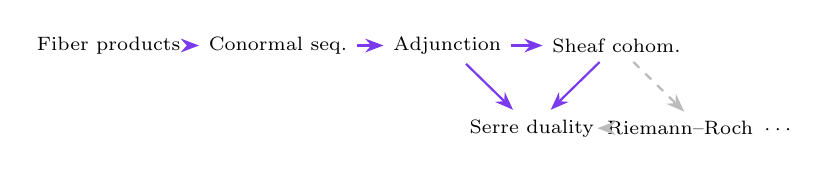
\begin{tikzpicture}[x=2.15cm, y=1.05cm, font=\scriptsize,
    arr/.style={-{Stealth}, chalkpurple, thick},
    darr/.style={-{Stealth}, chalkmuted, thick, dashed}]
    \node (fp)  at (0, 0)    {Fiber products};
    \node (cs)  at (1, 0)    {Conormal seq.};
    \node (adj) at (2, 0)    {Adjunction};
    \node (sc)  at (3, 0)    {Sheaf cohom.};
    \node (sd)  at (2.5,-1)  {Serre duality};
    \node (rr)  at (3.5,-1)  {Riemann--Roch\enspace$\cdots$};
    \draw[arr]  (fp)  -- (cs);
    \draw[arr]  (cs)  -- (adj);
    \draw[arr]  (adj) -- (sc);
    \draw[arr]  (adj) -- (sd);
    \draw[arr]  (sc)  -- (sd);
    \draw[darr] (sd)  -- (rr);
    \draw[darr] (sc)  -- (rr);
  \end{tikzpicture}
  \end{center}

  \medskip

  The residue exact sequence $+$ long exact cohomology sequence $+$
  Serre duality on $X$ and $Y$ together imply
  \textbf{Riemann--Roch for divisors} — the natural next destination.
\end{frame}

\end{document}
